\documentclass[main.tex,fontsize=8pt,paper=a4,paper=portrait,DIV=calc,]{scrartcl}
% Document
\usepackage[T1]{fontenc}
\usepackage[utf8]{inputenc}
\usepackage[dvipsnames]{xcolor}
\usepackage[nswissgerman,english]{babel} 
\usepackage{hyperref}
\renewcommand{\familydefault}{\sfdefault}

% Format
\usepackage[top=5mm,bottom=1mm,left=5mm,right=5mm]{geometry}
%\setlength{\headheight}{\baselineskip}
%\setlength{\headsep}{0mm}

%\usepackage{scrlayer-scrpage}
%\clearpairofpagestyles
%\chead{{\bfseries\TITLE, \AUTHOR, \pagename~\thepage}}

%\addtokomafont{pagehead}{\upshape}

\usepackage{multicol}
\setlength{\columnsep}{2mm}
\setlength{\columnseprule}{0.1pt}

% Math
\usepackage{amsmath}
\usepackage{amssymb}
\usepackage{amsfonts}

% Code
\usepackage{fancyvrb, etoolbox, listings, xcolor}
%\usemintedstyle{bw}

%\newminted[shell]{bash}{
%fontsize=\footnotesize,
%fontfamily=tt,
%breaklines=true,
%frame=single,
%framerule=0.1pt,
%framesep=2mm,
%tabsize=2
%}
%\newminted{css}{
%breaklines=true,
%tabsize=4,
%autogobble=true,
%escapeinside=||,
%stripall=true,
%stripnl=true,
%}

    \definecolor{lightgray}{rgb}{0.95, 0.95, 0.95}
    \definecolor{darkgray}{rgb}{0.4, 0.4, 0.4}
    \definecolor{purple}{rgb}{0.65, 0.12, 0.82}
    \definecolor{ocherCode}{rgb}{1, 0.5, 0} % #FF7F00 -> rgb(239, 169, 0)
    \definecolor{blueCode}{rgb}{0, 0, 0.93} % #0000EE -> rgb(0, 0, 238)
    \definecolor{greenCode}{rgb}{0, 0.6, 0} % #009900 -> rgb(0, 153, 0)
    \definecolor{teal}{rgb}{0.0, 0.5, 0.5}

\lstdefinestyle{code}{
    identifierstyle=\color{black},
    keywordstyle=\color{blue}\bfseries\small,
    ndkeywordstyle=\color{greenCode}\bfseries\small,
    stringstyle=\color{ocherCode}\ttfamily\small,
    commentstyle=\color{teal}\ttfamily\textit\small,
    basicstyle=\ttfamily\small,
    breakatwhitespace=false,         
    breaklines=true,                 
    captionpos=b,                    
    keepspaces=true,                 
    showspaces=false,                
    showstringspaces=false,
    showtabs=false,                  
    tabsize=2,
    belowskip=-5pt
}



% Images
\usepackage{graphicx}
\newcommand{\pic}{\includegraphics[scale=0.3]}
\graphicspath{{Screenshots/}{../Screenshots}}
\makeatletter
\def\pictext#1#2{%
    \@ifnextchar[{%
    \pictext@iiiii{#1}{#2}%
    }{%
      \pictext@iiiii{#1}{#2}[0.5,0.4,0.3]% Default is 5
    }%
}
\def\pictext@iiiii#1#2[#3,#4,#5]{\begin{minipage}{#3\textwidth}\includegraphics[scale=#4]{#1}\end{minipage}\begin{minipage}{#5\textwidth}#2\end{minipage}}
\def\minipg#1#2{%
    \@ifnextchar[{%
    \minipg@iiii{#1}{#2}%
    }{%
      \minipg@iiii{#1}{#2}[0.3,0.6]% Default is 5
    }%
}
\def\minipg@iiii#1#2[#3,#4]{\vspace{0.8mm}\begin{minipage}{#3\textwidth}#1\end{minipage}\begin{minipage}{#4\textwidth}#2\end{minipage}{\vspace{0.8mm}}}
\makeatother

%\newenvironment{minty}[2]% environment name
%{% begin code
%  \begin{minipage}{#1}
%  \begin{minted}{#2}
%}%
%{% end code
%  \end{minted}
%  \end{minipage}
%  \end{minty}\ignorespacesafterend
%} 

% Smaller Lists
\usepackage{enumitem}
\setlist[itemize,enumerate]{leftmargin=3mm, labelindent=0mm, labelwidth=1mm, labelsep=1mm, nosep}
\setlist[description]{leftmargin=0mm, nosep}
\setlength{\parindent}{0cm}

% Smaller Titles
\usepackage[explicit]{titlesec}

%% Color Boxes
\newcommand{\sectioncolor}[1]{\colorbox{black!60}{\parbox{0.989\linewidth}{\color{white}#1}}}
\newcommand{\subsectioncolor}[1]{\colorbox{black!50}{\parbox{0.989\linewidth}{\color{white}#1}}}
\newcommand{\subsubsectioncolor}[1]{\colorbox{black!40}{\parbox{0.989\linewidth}{\color{white}#1}}}
\newcommand{\paragraphcolor}[1]{\colorbox{black!30}{\parbox{0.989\linewidth}{\color{white}#1}}}
\newcommand{\subparagraphcolor}[1]{\colorbox{black!20}{\parbox{0.989\linewidth}{\color{white}#1}}}

%% Title Format
\titleformat{\section}{\vspace{0.5mm}\bfseries}{}{0mm}{\sectioncolor{\thesection~#1}}[{\vspace{0.5mm}}]
\titleformat{\subsection}{\vspace{0.5mm}\bfseries}{}{0mm}{\subsectioncolor{\thesubsection~#1}}[{\vspace{0.5mm}}]
\titleformat{\subsubsection}{\vspace{0.5mm}\bfseries}{}{0mm}{\subsubsectioncolor{\thesubsubsection~#1}}[{\vspace{0.5mm}}]
\titleformat{\paragraph}{\vspace{0.5mm}\bfseries}{}{0mm}{\paragraphcolor{\theparagraph~#1}}[{\vspace{0.5mm}}]
\titleformat{\subparagraph}{\vspace{0.5mm}\bfseries}{}{0mm}{\subparagraphcolor{\thesubparagraph~#1}}[{\vspace{0.5mm}}]

%% Title Spacing
\titlespacing{\section}{0mm}{0mm}{0mm}
\titlespacing{\subsection}{0mm}{0mm}{0mm}
\titlespacing{\subsubsection}{0mm}{0mm}{0mm}
\titlespacing{\paragraph}{0mm}{0mm}{0mm}
\titlespacing{\subparagraph}{0mm}{0mm}{0mm}

%% format cells
\usepackage[document]{ragged2e}
\usepackage{array, makecell}
\renewcommand{\arraystretch}{2}
\newcommand{\mc}{\makecell[{{m{1\linewidth}}}]}



\begin{document}
\tableofcontents

\newcommand{\TITLE}{Secure Software}
\newcommand{\AUTHOR}{Fabio Lenherr}
\setcounter{tocdepth}{1}

\section{Secure Software Principles}
\textcolor{Cyan}{Rather than trying to solve objectives in cyber security, you should have expectations of your software in terms of security.}

\subsection{CVSS Common Vulnerability Scoring System}
\begin{itemize}
  \item \textcolor{red}{High}\newline
    Heartbleed, log4j etc\newline
    often not noticeable, concealed
  \item \textcolor{blue}{Medium}\newline
    unclear if it can be exploited
  \item \textcolor{green}{Low}\newline
    typical problems like outdated tls certificate
\end{itemize}

\subsection{Low-hanging fruits first}
\textcolor{teal}{Before we go ahead and tackle the biggest issues, we can solve a lot of problems by making sure that we do not fail at the basics.}\newline
In other words, first try to solve the easy things.

\subsection{80\%/20\% Problem}
\begin{itemize}
\item \textcolor{purple}{Secure the weakest link}\newline
  A boomer might not know about phishing attacks, protect said user against doing something dumb!
\item \textcolor{purple}{Practice defense in depth}\newline
  Use multiple security layers, often 1 is not enough
\item \textcolor{purple}{Fail secure}\newline
  In terms of an error, don't just dump all information to some random person, eg. don't leak credit card information if the information is not 100\% correct.
\item \textcolor{purple}{Follow the principle of least privilege}\newline
  Don't give random people access to things they don't need
\item \textcolor{purple}{To Compartmentalize}\newline
  Try to categorize tasks, this makes it easier for people to get access to something.
\item \textcolor{purple}{Keep it simple}\newline
  Try to keep it as simple as possible
\item \textcolor{purple}{Promote privacy}\newline
  Handle privacy of users appropriately
\item \textcolor{purple}{Remember that hiding secrets is hard}
  In other words, security by obscurity is a novel practice and doesn't really work
\item \textcolor{purple}{Be reluctant to trust}
\item \textcolor{purple}{Use your community resources}
\end{itemize}

\section{Threat Models \& Mitigations}
\subsection{The 4 Questions}
\begin{enumerate}
\item \textcolor{purple}{What are we working on?}\newline
  \begin{itemize}
  \item \textcolor{black}{Define scope and context}
  \item \textcolor{black}{Description of requirements and design}
  \end{itemize} 
\item \textcolor{purple}{What can go wrong?}\newline
  Anciticapte potential issues (think like the attacker)
\item \textcolor{purple}{What are we going to do about it?}\newline
  Define mitigations
\item \textcolor{purple}{Did we do a good job?}\newline
  Reflection and confirmation
\end{enumerate} 

\subsection{Methodology for Threat Risk Modeling}
\begin{enumerate}
\item \textcolor{purple}{Identify security objectives with a focus on:}\newline
 \begin{itemize}
 \item \textcolor{black}{sensitive information stored on device}
 \item \textcolor{black}{third party libraries used}
 \item \textcolor{black}{loss of repudation derived from misuse of the application}
 \end{itemize} 
\item \textcolor{purple}{Break down the application features, i.e. decomposition of the application into small feature sets with the goal to identify security impact}
\item \textcolor{purple}{Identification of related threats and vulnerabilities in implementation}
\end{enumerate} 

\subsection{Process Steps}
\begin{enumerate}
\item \textcolor{purple}{Identity Assets}\newline
What do we own and what do we want to protect? Not everything is worth protecting!
\item \textcolor{purple}{Create an architecture overview}\newline
  Simple diagrams which include application, subsystems, trust boundaries and data flow
\item \textcolor{purple}{Decompose the application}\newline
  The structure of your application -> network model, API, etc that can lead to potential vulnerabilities
\item \textcolor{purple}{Identify the threats}\newline
  From the attackers perspective, try to find loopholes etc to attack your application and \emph{document them}
\item \textcolor{purple}{Document the threats}\newline
\item \textcolor{purple}{Rate the threats} \newline
  Rate the threats according to \emph{likelihood, impact damage (reputation, cost), damage of migitation (cost, annoyance or work)}
\end{enumerate} 

\subsection{Why?}
The reason we do all this is that the following 3 groups have the these benefits: 
\begin{itemize}
\item \textcolor{purple}{Developers}\newline
  \begin{itemize}
  \item \textcolor{black}{Know potential threats and develop with them in mind}
  \item \textcolor{black}{priorization of threats to proper mitigations can be taken}
  \end{itemize} 
\item \textcolor{purple}{Penetration Testers}\newline
  \begin{itemize}
  \item \textcolor{black}{Makes sure penetration testers don't waste time testing things that don't matter to you}
  \item \textcolor{black}{Have a decent idea where to start}
  \end{itemize} 
\item \textcolor{purple}{Management}\newline
  \begin{itemize}
  \item \textcolor{black}{Know the risks in their language -> cost}
  \item \textcolor{black}{Don't make stupid decisions against developers etc since they don't understand IT}
  \end{itemize} 
\end{itemize} 

\subsection{STRIDE}
\begin{itemize}
\item \textcolor{purple}{Spoofing}\newline
Using a false identity to gain access to a system.\newline
\textcolor{green}{Mitigation: Authentication} Cookies, Signatures, updates TLS
\item \textcolor{purple}{Tampering}\newline
unauthorized changes/manipulation of data\newline
\textcolor{green}{Mitigation: Integrity} ACLs, Digital Signatures
\item \textcolor{purple}{Repudation}\newline
The ability to deny having performed an attack,\newline
\textcolor{green}{Mitigation: Nonrepudation} Secure logging and auditing, Digital Signatures
\item \textcolor{purple}{Impersonation}\newline
unauthorized revelation of classified(PROPRIETARY) private information.\newline
\textcolor{green}{Mitigation: Confidentiality} Encryption, ACLS
\item \textcolor{purple}{Denial of Service}\newline
Prevent or restrict access to a service by flooding it.\newline
\textcolor{green}{Mitigation: Availability} ACLs, Filtering, Quotas
\item \textcolor{purple}{Elevation of Privilege}\newline
Gaining unauthorized privileges on a system. For example: becoming root as regular user\newline
\textcolor{green}{Mitigation: Authorization} ACLs, Group or role membership, privilege ownership, input validation
\end{itemize} 

\subsubsection{Stride and Thread Modeling}
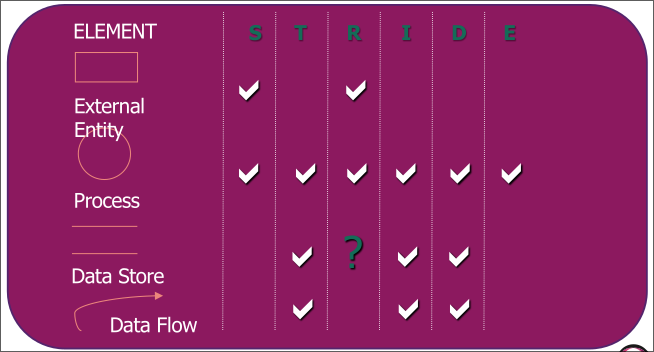
\includegraphics[scale=0.4]{2023_03_02_10_46_31.png}

\subsection{Attack Tree}
This is a list of attacks that can lead to another. This can help with attacks that are \emph{not obvious}.\newline
\textcolor{puple}{Attack trees are complementary to threat modeling}\newline
\textcolor{red}{Here an example of how they work:}\newline
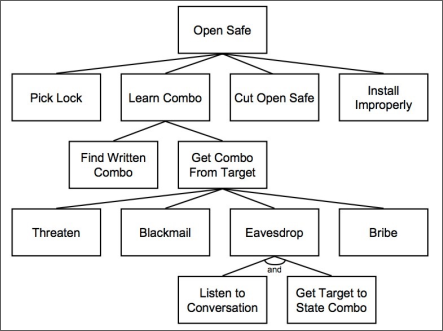
\includegraphics[scale=0.4]{2023_03_02_11_20_47.png}
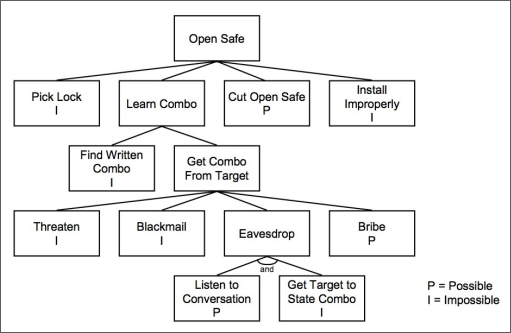
\includegraphics[scale=0.4]{2023_03_02_11_22_00.png}\newline
\textcolor{purple}{Add labels for possible and impossible actions}\newline
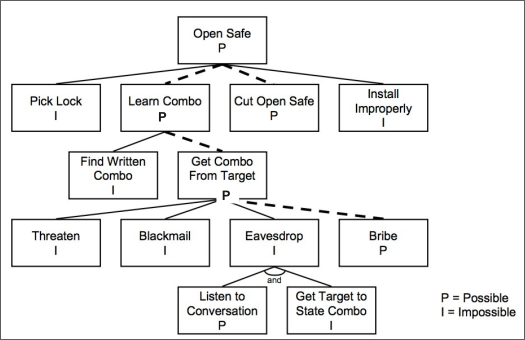
\includegraphics[scale=0.4]{2023_03_02_11_22_15.png}
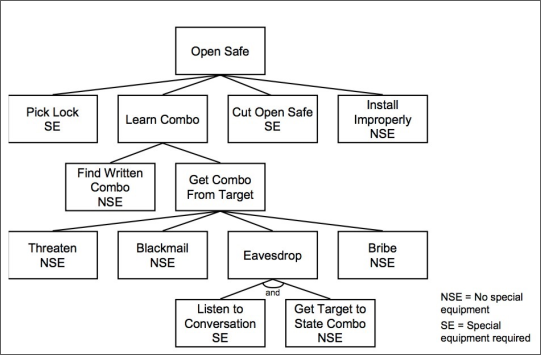
\includegraphics[scale=0.4]{2023_03_02_11_22_25.png}\newline
\textcolor{purple}{Propagate the labels up so possible things are closer, after that \emph{define used tools for the actoins}}\newline
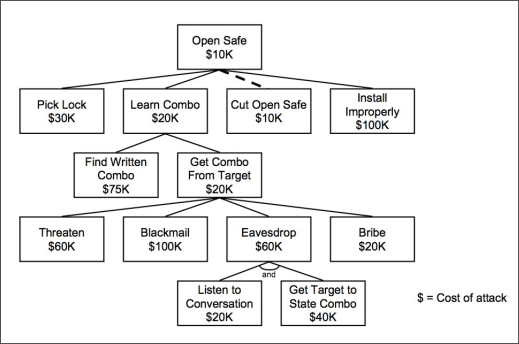
\includegraphics[scale=0.4]{2023_03_02_11_23_15.png}
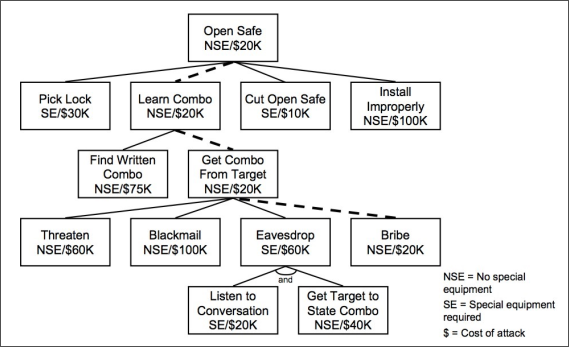
\includegraphics[scale=0.4]{2023_03_02_11_23_34.png}\newline
\textcolor{purple}{Define monetary costs for the attack and \emph{mark the route with least cost and the least tools used}}

\subsection{Risk Management Acitivies}
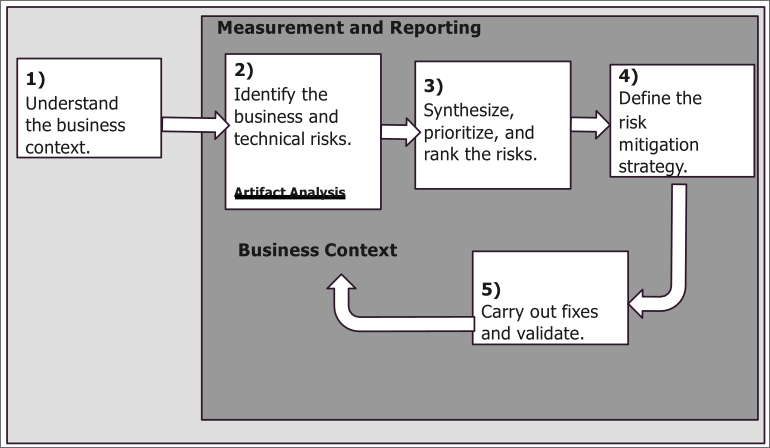
\includegraphics[scale=0.4]{2023_03_02_11_13_47.png}\newline

\section{Software bugs and unexpected behavior}

\section{Web Security}

\section{Reverse Engineering}

\section{Secure Software Lifecycle}

\section{Mobile Security}

\section{Security Testing}

\section{Bug Bounty}

\section{Software Security Assurance}

\section{Summary}

\end{document}
